\section{Thiết kế hệ thống}
\subsection{Thiết kế cơ sở dữ liệu sử dụng cho màn chơi}
\hspace*{0.5cm} Cơ chế chơi chính của trò chơi là sử dụng một Cơ sở dữ liệu do game cung cấp, tận dụng thông tin thu thập được từ cơ sở dữ liệu cũng như sử dụng chính các câu truy vấn này để thực hiện các hành động trong màn chơi, khi đối đầu với kẻ thù. Một trong những thứ không thể thiếu của game là cơ sở dữ liệu của trò chơi. Người chơi sẽ sử dụng các câu truy vấn SQL để khai thác tối đa SQL, tìm được mục tiêu và tiêu diệt chúng. Bản chất của Cơ sở dữ liệu sử dụng trong game được xem như một phần của giao diện, là cầu nối để người chơi tương tác với game, không được sử dụng để lưu trữ thông tin dài hạn như các hệ thống sử dụng cơ sở dữ liệu khác. Trạng thái của màn chơi hiện tại cũng ánh xạ một phàn vào trạng thái của Cơ sở dữ liệu sử dụng trong màn chơi\\
\hspace*{0.5cm} Để thiết kế và hiện thực cơ sở dữ liệu để đưa vào trò chơi cho người chơi tương tác, nhóm trải qua các giai đoạn tương tự với các giai đoạn của việc thiết kế cơ sở dữ liệu thường được áp dụng.
\subsubsection{Giai đoạn 1: Thu thập và phân tích yêu cầu nghiệp vụ}
\hspace*{0.5cm} Căn cứ vào các yêu cầu chức năng, phi chức năng và cơ chế gameplay chính của trò chơi, nhóm cũng thu thập, phân tích và đúc kết được một số yêu cầu cho cơ sở dữ liệu của màn chơi.
\begin{itemize}
	\item Thực thể trong màn chơi là thực thể sẽ được tồn tại với một mã định danh (ID) là chuỗi 8 ký tự, bao gồm chữ cái thường hoặc chữ số, đi kèm với đó là tên của thực thể và mô tả của thực thể đó, tên và mô tả có thể không có dữ liệu. Thực thể có thể là Người chơi, Quái vật, bộ phận quái vật, mỗi thực thể không thể mang 2 loại, ví dụ như người chơi không thể là quái vật. Thực thể có thể không là 1 trong 3 loại trên, nó có thể là các vật thể tồn tại trong môi trường của màn chơi và khu vực chiến đấu.
	\item Người chơi là dạng thực thể sẽ được điều khiển của người dùng. Người chơi gồm trạng thái hiện tại của người chơi, bao gồm HP hiện tại cũng như HP tối đa, cùng cấp độ và Kinh nghiệm hiện tại của người chơi. Người chơi cũng có một bộ Thông số hiện tại, thông số tối đa để người chơi có thể theo dõi. Người chơi cũng có các trạng thái về hiệu ứng hiện tại, bao gồm hiệu ứng lửa, độc, mù, băng, hiệu ứng câu lệnh,.... Người chơi cũng có Inventory chứa các vật phẩm cũng như các slot trang bị dành cho người chơi.
	\item Vật phẩm của trò chơi là các vật phẩm được sử dụng trong trò chơi và màn chơi. Vật phẩm phải có một mã định danh riêng biệt cho vật phẩm là một chuỗi có 7 kí tự gồm số và chữ cái thường, cùng tên và mô tả, cũng như là độ hiếm của trang bị. Vật phẩm có thể là trang bị, vật phẩm sử dụng được, hoặc không thuộc loại nào. Vật phẩm chỉ có thể là trang bị, hoặc là vật phẩm, không thể vừa là trang bị vừa là vật phẩm tiêu thụ được. Vật phẩm có thể nằm trong Inventory hoặc không, Có thể có nhiều vật phẩm nằm trong Inventory của người chơi.
	\item Trang bị là một loại vật phẩm, người chơi có các slot trang bị nhất định. Mỗi món trang bị sẽ có từ 1-3 traits, được tổng hợp lại cho người chơi để xét mỗi khi quái vật tấn công hoặc ảnh hưởng của môi trường. Mỗi món trang bị chỉ có thể ở trong kho đồ với số lượng là 1. Các món trang bị có thể thuộc các loại khác nhau nhưng nó vẫn cùng chung một cấu trúc bộ chỉ số. Các món trang bị có các chỉ số cơ bản là cấp độ trang bị hiện tại và yêu cầu cấp độ người chơi để có thể trang bị được món trang bị. Ngoài ra, trang bị cũng mang bộ chỉ số hiện tại. Mỗi món trang bị tồn tại một đòn đánh thường và các kỹ năng (nếu có). Các kỹ năng là riêng biệt với nhau, mỗi kỹ năng phân biệt nhau bằng một chuỗi 6 ký tự theo dạng "Pxxxxx" với x là các chữ số hoặc chữ cái in hoa, một kỹ năng có thể được nhiều trang bị sử dụng. Các kỹ năng này đều có trạng thái hồi kỹ năng, người chơi cần đưa ra các chiến lược sử dụng hợp lý. Các kỹ năng bao gồm tên, mô tả và bộ thông số tính thêm khi sử dụng. Khi thực hiện đòn đánh với kỹ năng, hệ thống sẽ tổng hợp các tham số cơ bản của trang bị và tham số cộng thêm của đòn đánh. Mỗi kỹ năng cũng sẽ có tối đa 2 traits để xét độ hiệu quả của kỹ năng, trait này phải có ít nhất 1 trait trong bộ trait của trang bị.
	\item Vật phẩm sử dụng được là vật phẩm người chơi có thể sử dụng được, mang lại các lợi ích cho người chơi. Các thông số của món vật phẩm bao gồm: Hồi máu, giảm hiệu ứng, và các thông số tăng cường như tấn công, phòng thủ và nhanh nhẹn.
	\item Bộ thông số được sử dụng chung cho Người chơi, quái vật, trang bị, kỹ năng quái vật và của trang bị. Cấu trúc khoá bao gồm mã định danh của thực thể, hoặc trang bị, hoặc mã kỹ năng của quái vật, hoặc mã trang bị + index của kỹ năng, và mục đích sử dụng bộ thông số này. Mục đích sử dụng được viết theo dạng xâu, ví dụ như "Current" chỉ thông số hiện tai, "Max" chỉ thông số tối đa, "Modify" chỉ thông số sẽ thay đổi (thường được sử dụng cho các kỹ năng của quái vật và kỹ năng của trang bị được trang bị trong slot). Thông số bao gồm chỉ số tấn công, phòng thủ, nhanh nhẹn và các sát thương hiệu ứng tấn công và kháng hiệu ứng, bao gồm hiệu ứng lửa, độc, mù, băng, hiệu ứng câu lệnh,... Với một chủ và mục đích sử dụng chỉ có duy nhất 1 bộ thông số, các thực thể có thể phải có 1 bộ thông số với các mục đích khác nhau. 
	\item Quái vật là thực thể, là kẻ thù của người chơi. Quái vật có các thông số về Level, Độ trà trộn sẽ được sử dụng để tạo bản sao. Quái vật vẫn có bộ thông số hiện tại tương tự với bộ thông số đã được đề cập ở trên. Quái vật chỉ thuộc một loại Quái vật, một Loại Quái vật có thể có nhiều quái vật thuộc loại. Loại Quái vật gồm có tên loại là duy nhất. Mỗi Loại quái vật còn đi kèm một bộ gồm một số kỹ năng của quái vật. Mỗi kỹ năng có thể thuộc nhiều loại quái vật khác nhau, mỗi kỹ năng bao gồm mã kỹ năng là duy nhất là một chuỗi gồm 6 ký tự theo dạng "Exxxx", với x là các chữ số hoặc chữ cái viết hoa, tên và mô tả, các khả năng đặc biệt, hồi chiêu chuẩn của kỹ năng cũng như bộ thông số của kỹ năng quái vật. Quái vật có thể chọn một số kỹ năng của loại quái vật làm kỹ năng cho mình (quái vật không nhất thiết phải chọn toàn bộ kỹ năng tương ứng với loại quái vật). Loại Quái vật cũng có tối đa 1 Trait được sử dụng cho việc xét ảnh hưởng của môi trường. Kỹ năng quái vật cũng có một số trait để có thể xét khắc chế khi tấn công người chơi. 
	\item Mỗi quái vật tồn tại nhờ một số bộ phận chí mạng gắn trên người, các bộ phận chí mạng này có thể là các bộ phận không thuộc quái vật nào. Quái vật nếu không còn bộ phận thật nào còn tồn tại sẽ bị tiêu diệt. Bộ phận chí mạng cũng là một thực thể của trò chơi, nghĩa là nó vẫn có mã định danh, tên và mô tả. Ngoài ra còn các thông số trạng thái như máu hiện tại, máu tối đa, loại bộ phận (có thể là tay súng, giáp, kiếm) hỗ trợ cho việc xác định. Các bộ phận này cũng có từ 1-3 traits để xét khắc chế khi người chơi tấn công. 
	\item Traits là loại phẩm chất được sử dụng để xét khắc chế bởi đòn đánh của người chơi, quái vật, ảnh hưởng của môi trường. Trait có thể tồn tại ở bộ phận quái vật, loại quái vật, kỹ năng quái vật, trang bị, kỹ năng trang bị của người chơi. Trait bao gồm tên trait phân biệt, kèm mô tả trait đó. Một trait có thể là khắc chế của 0 hoặc nhiều trait khác, hoặc cũng có thể bị khắc chế của 0 hoặc nhiều trait.
	\item Để cung cấp clue cho người chơi, ngoài phản ứng của quái vật và hiệu ứng trả về của đòn đánh (Super/Not Really Effective), cơ sở dữ liệu của game cần có các bảng về các thông tin về quái vật như Ngoại hình, hội thoại của quái vật. Ngoại hình của quái vật có khoá bao gồm mã định danh thực thể và category của ngoại hình, kèm với mô tả ngoại hình. Mỗi mã thực thể có một hội thoại riêng. So với tương tác trong game thì các hội thoại và ngoại hình này có thể có sự thay đổi, ví dụ như đổi giá trị, mã hoá, cất bớt một số điểm,...
	\item Để có thể thực hiện các hành động như tấn công, sử dụng vật phẩm,... Có các bảng hỗ trợ để người chơi có thể đưa các tham số vào. Bảng attack bao gồm các tham số là mã thực thể mục tiêu, mã trang bị sử dụng (cả 2 được gộp thành một khoá, 2 tham số không được null), cùng với index của kỹ năng, nếu index bằng 0 hoặc null nghĩa là sử dụng đòn đánh thường của vũ khí. Bảng use bao gồm mã trang bị. Người chơi cần chèn các tham số vào bảng thì hành động mới có thể được thực thi.
	
\end{itemize}
\subsubsection{Giai đoạn 2: Thiết kế ý niệm của cơ sở dữ liệu}
\hspace*{0.5cm} Một trong những thứ không thể thiếu của game là schema của trò chơi. Người chơi sẽ sử dụng các câu truy vấn SQL để khai thác tối đa SQL, tìm được mục tiêu và tiêu diệt chúng.
\begin{figure}[H]
	\centering
	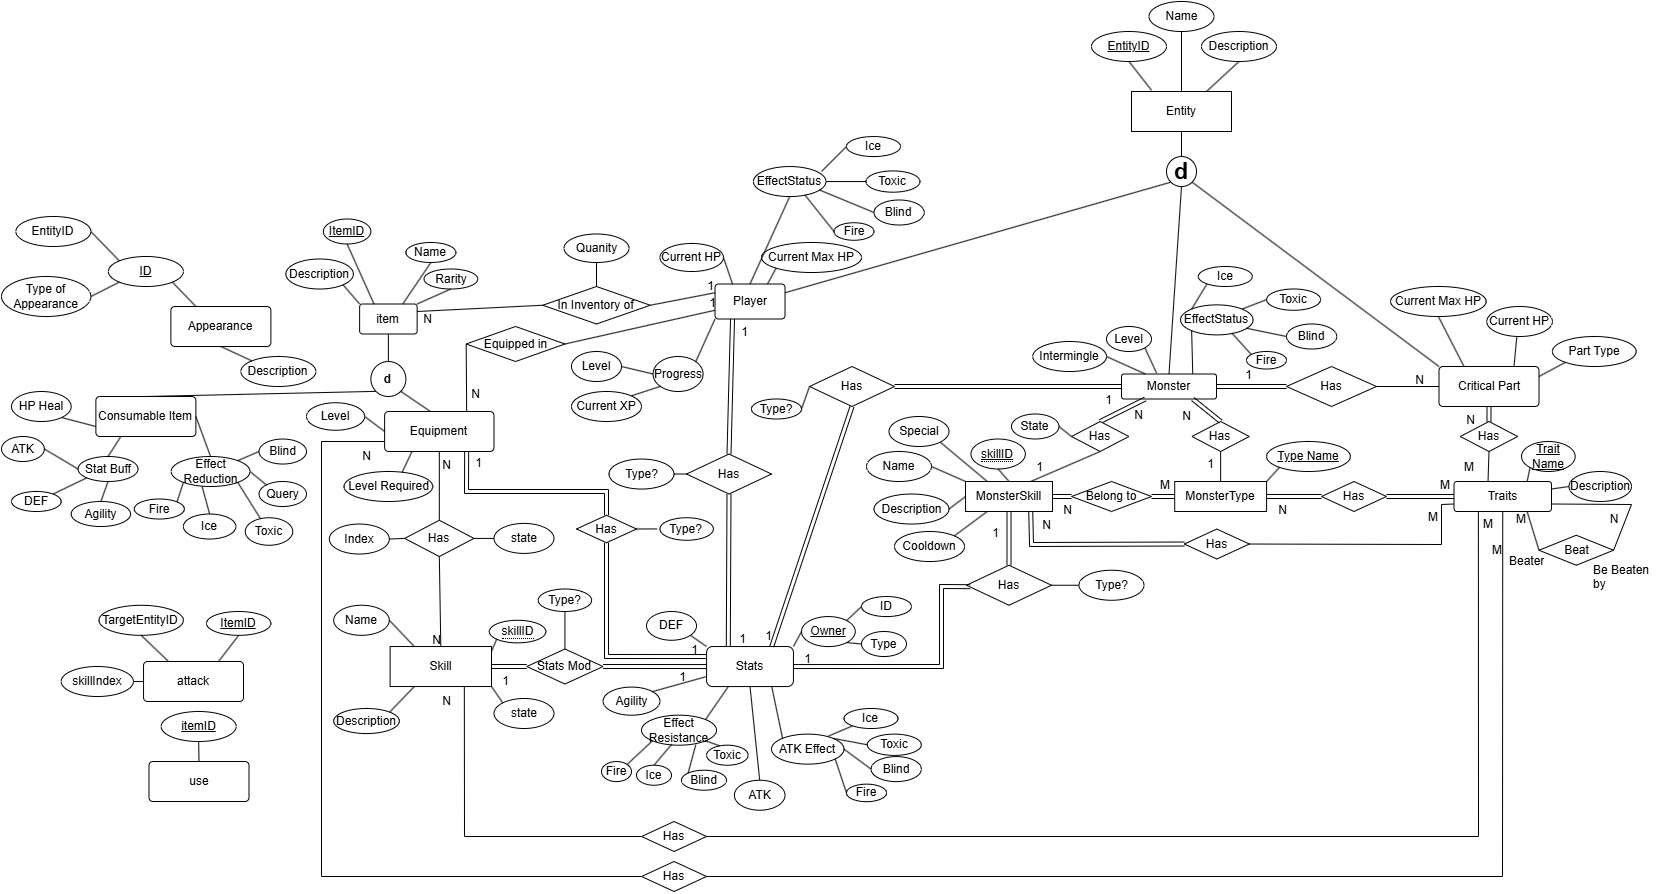
\includegraphics[width=\textwidth]{Images/eerd.jpg}
	\vspace{0.5cm}
	\caption{Mô hình thực thể - quan hệ của cơ sở dữ liệu của màn chơi}
\end{figure}

\subsubsection{Giai đoạn 3: Lựa chọn Hệ quản trị cơ sở dữ liệu}
\hspace*{0.5cm} Ở giai đoạn này, cần lựa chọn Hệ quản trị cơ sở dữ liệu phù hợp với các tiêu chí đặt ra để game hoạt động đúng mục đích, đúng kỳ vọng. Để có thể xử lý câu truy vấn được nhập từ User, nhóm đã nghiên cứu các giải pháp sao cho có thể nhận câu SQL người chơi đã nhập, xử lý và trả kết quả về cho hệ thống xử lý và đưa ra các phản ứng của game. Một số tiêu chí được đưa ra:
\begin{itemize}
	\item \textbf{Về mặt kỹ thuật: } Hệ quản trị có thể nhận và xử lý câu truy vấn được nhập từ người dùng bằng ngôn ngữ SQL; Tốc độ xử lý đủ nhanh để trả kết quả hoặc phản ứng của game lên trên màn hình; Hệ quản trị nên được đặt trong nội bộ máy tính; Tính di động cao, Hệ quản trị vầ game có thể được chạy trên các nền tảng phần cứng khác nhau;
	\item \textbf{Về mặt phi kỹ thuật: } Tập trung chủ yếu vào chi phí mua các phần mềm để tích hợp việc xử lý SQL giữa Hệ quản trị cơ sở dữ liệu và ứng dụng game. 
\end{itemize}

\hspace*{0.5cm }Có rất nhiều hướng tiếp cập khác nhau. Nhưng nhóm cũng lựa chọn một số hướng tiếp cận nhất định.
\paragraph {Hướng tiếp cận sử dụng MySQL bằng cách thiết lập máy chủ cục bộ chạy trong máy người chơi}
\hspace*{0.5cm} Hướng tiếp cận này sử dụng một hệ quản trị cơ sở dữ liệu như MySQL hoặc tương tự và được chạy trong như một tiến trình máy chủ cục bộ độc lập và việc giao tiếp giữa Cơ sở dữ liệu và game là thông qua việc kết nối Hệ cơ sở dữ liệu thông qua localhost và một port nhất định. Việc thiết lập một máy chủ cục bộ chạy MySQL là riêng biệt. Về phía Game Client chỉ cần tạo một class \textit{SQLConnector}, truyền vào các tham số rồi kết nối đến máy chủ cục bộ đã thiết lập. Các câu truy vấn sẽ được connector này gọi truy vấn đến máy chủ cục bộ, kết quả hoặc lỗi cũng sẽ do connector này nhận và xử lý, truyền sang các lớp khác.\\
\begin{figure}[H]
	\centering
	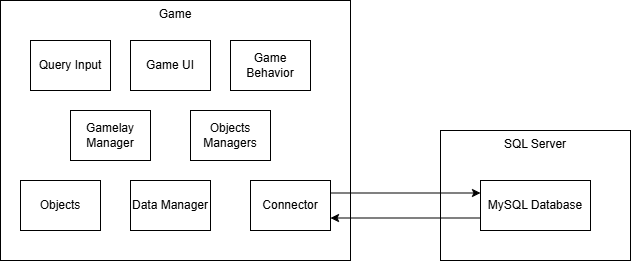
\includegraphics[width=\textwidth]{Images/SQLLocalServer.png}
	\vspace{0.5cm}
	\caption{Mô hình cấu trúc của hướng giải pháp chạy SQL Server trên Local}
\end{figure}
\hspace*{0.5cm} Với việc sử dụng một process riêng, ta có thể tuỳ biến process theo dạng Hệ cơ sở dữ liệu SQL nào đều được, bao gồm MySQL, PostgreSQL,... Miễn là ta lựa chọn thư viện Database Client cho Connector phù hợp là được. Ta sẽ có toàn bộ chức năng như một hệ cơ sở dữ liệu thuần tuý, ta có thể thiết lập các stored procedure, function, thiết lập các quyền cho các user khác nhau cũng như nhiều tính năng hỗ trợ hơn.\\
\hspace*{0.5cm} Tuy nhiên, với việc sử dụng một process riêng và có sử dụng port. Nếu không xử lý port hợp lý, port mà process chiếm dụng sẽ không được sử dụng cho mục đích khác nữa. Hơn nữa, việc chạy localhost server bản chất vẫn là process, và nó có thể chấm dứt bởi trình quản lý tác vụ của hệ điều hành. Nếu mất đi kết nối với server local, game sẽ không thể thực thi các tác vụ có liên quan đến SQL, game sẽ không thể hoạt động và đó là điều không thể chấp nhận được. Hơn nữa, việc khởi chạy game đòi hỏi game cũng phải khởi chạy thêm tiến trình server. Cũng như khi cài đặt trò chơi, ta phải cài đặt thêm SQL Server. Khiến cho cấu trúc lủng củng, không nhất quán, đặc biệt là nếu SQL Server có sự cố thì game cũng không hoạt động được, dẫn đến chạy không ổn định.
\paragraph {Hướng tiếp cận xây dựng Hệ cơ sở dữ liệu SQLite ngay trong game}
\hspace*{0.5cm} Thay vì sử dụng một process riêng biệt, hướng tiếp cận này sử dụng SQLite, là một hệ cơ sở dữ liệu gọn nhẹ, có khả năng nhúng vào các ứng dụng khác. Đây là một ưu điểm lớn của SQLite khi nó có thể thực hiện các câu truy vấn ngay trong lòng ứng dụng, giúp cho cấu trúc được nhất quán và hoạt động đồng nhất và ổn định.
\begin{figure}[H]
	\centering
	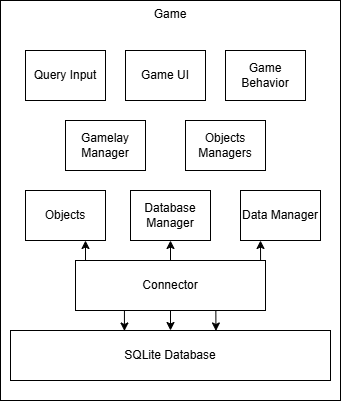
\includegraphics[width=\textwidth]{Images/SQLITE.png}
	\vspace{0.5cm}
	\caption{Cấu trúc game với Hệ cơ sở dữ liệu SQLite}
\end{figure}
\hspace{0.5cm} Cách thiết lập cũng khá đơn giản, chỉ cần một file .db, và một module connector để kết nối với cơ sở dữ liệu cục bộ, connector cũng đóng vai trò thực hiện các câu truy vấn từ hệ thống và người chơi. 
\hspace*{0.5cm} Tuy nó có sự tiện lơi và gọn nhẹ và dễ dàng nhúng vào các ứng dụng khác, nhưng đổi lại, nó phải hy sinh nhiều tính năng. Trên hết là việc nó không hỗ trợ ràng buộc khoá ngoại tham chiếu đến nhiều bảng. Nó không hỗ trợ cấp quyền cho người dùng, nên việc xử lý các câu truy vấn của người dùng sẽ phải thêm một số bước mới có thể cho ra kết quả như kỳ vọng. Ngoài ra, với việc không có stored procedure cũng là một thiệt thòi lớn cho những ai muốn sử dụng procedure.\\
\hspace*{0.5cm} Bỏ qua những khuyết điẻm mà giải pháp này còn tồn đọng, nhóm vẫn quyết định sử dụng giải pháp này vì tính nhất quán và đồng nhất với dự án. Các vấn đề phát sinh nhóm sẽ có những cách xử lý khác nhau.
\subsubsection{Giai đoạn 4: Thiết kế cơ sở dữ liệu luận lý}
\hspace*{0.5cm} Từ những yêu cầu và cơ sở dữ liệu luận lý, nhóm bắt đầu thiết kế cơ sở dữ liệu luận lý, thể hiện các quan hệ và các ràng buộc về khoá ngoại.
\begin{figure}[H]
	\centering
	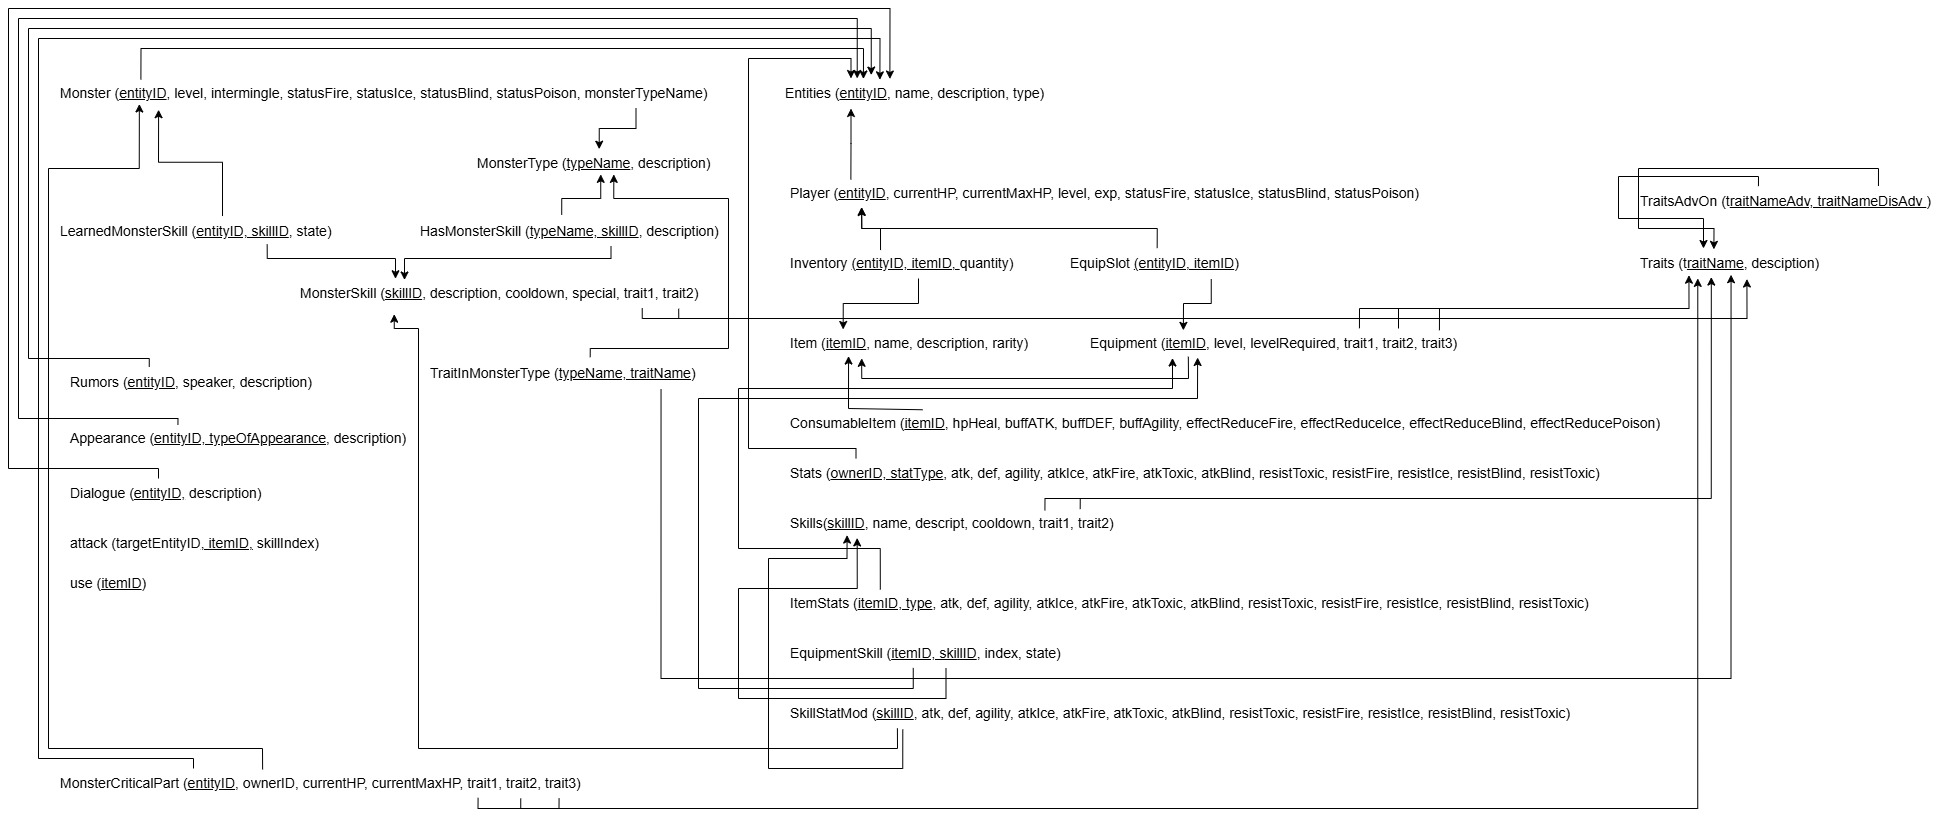
\includegraphics[width=\textwidth]{Images/rm.jpg}
	\vspace{0.5cm}
	\caption{Mô hình quan hệ - cơ sở dữ liệu luận lý trong màn chơi}
\end{figure}





\subsection{Luật xử lý dựa trên hành động của người chơi}
\hspace*{0.5cm} Trong quá trình chơi, khó mà tránh khỏi việc người chơi có những hành vi cố ý tác động đến schema, nếu không xử lý hợp lý sẽ gây tình trạng màn chơi bị rối loạn, cũng như có thể dẫn đến mất ổn định game. Luôn nhớ rằng Schema chỉ là Playground của game, các object của game chỉ được quản lý bởi hệ thống, nên việc xử lý phải mang tính răn đe, cho người chơi nhớ được mọi hành vi của bản thân đều có thể mang lại hậu quả, tương tự với việc xử lý SQL trong công việc thực tế.\\

\hspace*{0.5cm} Với việc nhóm quyết định sử dụng SQLite và tích hợp thẳng vào game. Khiến nó bộc lộ hạn chế lớn: nó không hỗ trợ việc phân quyền. Vì vậy nhóm quyết định đặt ra các bộ quy tắc để xử lý ở mức DB Manager khi người chơi có các hành vi cụ thể với cấu trúc của cơ sở dữ liệu hoặc dữ liệu trong các bảng.
\subsubsection{Tạo, sửa, xoá bảng, trigger,...}
\hspace*{0.5cm} Hành vi tạo, sửa, xoá bảng hoặc các trigger của người chơi được xem là hành vi cấm. Song SQLite tích hợp vào Unity không hỗ trợ việc phân quyền và ngăn chặn các hành vi tạo, xoá, sửa bảng ở cấp Hệ quản trị cơ sở dữ liệu, nên việc xử lý này phải được thực hiện ở cấp ứng dụng, tức là game. Với mỗi câu truy vấn người chơi submit cho game, một module tên là SQLAnalyzer sẽ được gọi để kiểm tra xem câu lệnh có chứa các từ khoá như "CREATE", "DROP", "ALTER",... nếu có sẽ gọi báo lỗi và hiện lỗi lên trên màn hình và người chơi được phép nhập lại câu lệnh khác. 
\subsubsection{Thay đổi trạng thái của bảng}
Với các bảng khác nhau, sẽ có quy luật để game xử lý khác nhau cho mỗi thao tác, chèn thêm, cập nhật và xoá record trong một bảng nhất định.
\begin{longtable}{|p{3cm}|p{3cm}|p{3cm}|p{3cm}|}	
	\hline
	\textbf{Tên bảng} & \textbf{Insert} & \textbf{Update} & \textbf{Delete}\\
	\hline
	\endhead
	
	\hline
	\endfoot
	
	\hline
	Player & Game xoá các record rác & Game cập nhật lại các record bị sai & Game ngăn người chơi xoá record bằng trigger\\
	\hline
	Monster & Game giữ lại, không đổi, làm người chơi khó khăn hơn & Game cập nhật lại các record bị sửa & Game cho phép xoá, đổi lại cơ sở dữ liệu không tìm được mục tiêu, người chơi không thể xác định được mục tiêu\\
	\hline
	MonsterType & Không cho phép & Không cho phép & Không cho phép\\
	\hline
	MonsterSkill & Không cho phép & Không cho phép & Không cho phép\\
	\hline
	LearnedMonsterSkill & Cho phép chèn vào nhưng không có ý nghĩa & Cho phép chỉnh sửa nhưng không có ý nghĩa & Cho phép xoá nhưng không có ý nghĩa\\
	\hline
	HasMonsterSkill & Không cho phép & Không cho phép & Không cho phép\\
	\hline
	MonsterCriticalPart & Cho phép chèn vào nhưng sẽ gây khó cho người chơi & Game cập nhật lại các record bị sửa & Game cho phép xoá, đổi lại cơ sở dữ liệu không tìm được mục tiêu, người chơi không thể xác định được mục tiêu\\
	\hline
	Trait & Không cho phép & Không cho phép & Không cho phép\\
	\hline
	TraitAdvOn & Không cho phép & Không cho phép & Không cho phép\\
	\hline
	Entities & Cho phép chèn vào, không mang lại lợi ích cho người chơi, mà chỉ khiến cho bảng dữ liệu to ra & Không cho phép cập nhật & Cho phép xoá, nếu entity không phải là Player, Monster hay MonsterCriticalPart, vì đó được xem là Environmental Objects. Nếu xoá object trong môi trường có thể kích hoạt hiệu ứng của vật thể đó, hiệu ứng có thể mang lại lợi thế, bất lợi, thậm chí còn mang hậu quả nghiêm trọng.\\
	\hline 
	Item & Không cho phép & Không cho phép & Không cho phép\\
	\hline
	Equipment & Không cho phép & Không cho phép & Không cho phép\\
	\hline
	Skills & Không cho phép & Không cho phép & Không cho phép\\
	\hline
	EquipmentSkill & Không cho phép & Không cho phép & Không cho phép\\
	\hline
	ConsumableItem & Không cho phép & Không cho phép & Không cho phép\\
	\hline
	Inventory, EquipSlot & Cho phép chèn vào. Nhưng cho dù người chơi có chèn vào bao nhiêu record dữ liệu giả rồi sử dụng chúng trong hàm attack hoặc use đều vô hiệu. Schema tìm được ID trong quá trình xử lý câu lệnh nhưng đưa vào hệ thống game để thao tác mà không tìm ID cũng vô nghĩa, hệ thống sẽ thông báo đã không có gì xảy ra và lượt thao tác của người chơi kết thúc. Không như việc ID không đúng thì người chơi vẫn có cơ hội nhập lại, việc thêm ID giả vào sẽ mang lại hậu quả nghiêm trọng hơn cho người chơi. & Game cập nhật lại giá trị về trước khi bị thay đổi bởi người chơi & Cho phép xoá, nhưng sẽ mang lại bất lợi cho người chơi. Khi người chơi thực hiện hàm attack, use thì schema sẽ báo lỗi không tìm thấy id phù hợp, khi đó người chơi đến hết màn chơi không thể sử dụng hoặc tấn công bằng item đó nữa.\\
	\hline
	Các bảng Stats & Vẫn chèn đươc, nhưng không có ý nghĩa gì & Vẫn sửa được, không mang lại lợi ích gì & Vẫn xoá được, không mang lại lợi ích gì. \\
	\hline
	Các bảng Rumor, Appearance, Dialogue & Vẫn chèn đươc, nhưng không có ý nghĩa gì, có thể gây rối trong việc xác định mục tiêu & Vẫn sửa được, không mang lại lợi ích gì, có thể gây khó khăn cho người chơi & Vẫn xoá được, không mang lại lợi ích gì. Người chơi mất thông tin đó, có thể gây khó khăn vì có thể mất thông tin quan trọng.\\
	\hline
	
\end{longtable}
\subsubsection{Nhập vào nhiều câu truy vấn}
\hspace*{0.5cm} Mỗi lượt game chỉ chấp nhận một câu truy vấn từ người chơi. Trong trường hợp người chơi cố tình nhập nhiều câu lệnh theo đúng cấu trúc (các câu lệnh được ngăn cách nhau bằng dấu chấm phẩy ";") thì SQLAnalyzer sẽ phân tách thành các câu lệnh riêng và chọn câu lệnh được nhập vào đầu tiên để xử lý các bước tiếp theo. Đồng thời hiện thông báo người chơi đã nhập nhiều câu truy vấn trong một lượt, cũng như khung nhập câu truy vấn cũng đổi văn bản đã nhập thành câu lệnh đầu tiên.
\subsection{Cấu trúc module chính của Game}
\begin{figure}[H]
	\centering
	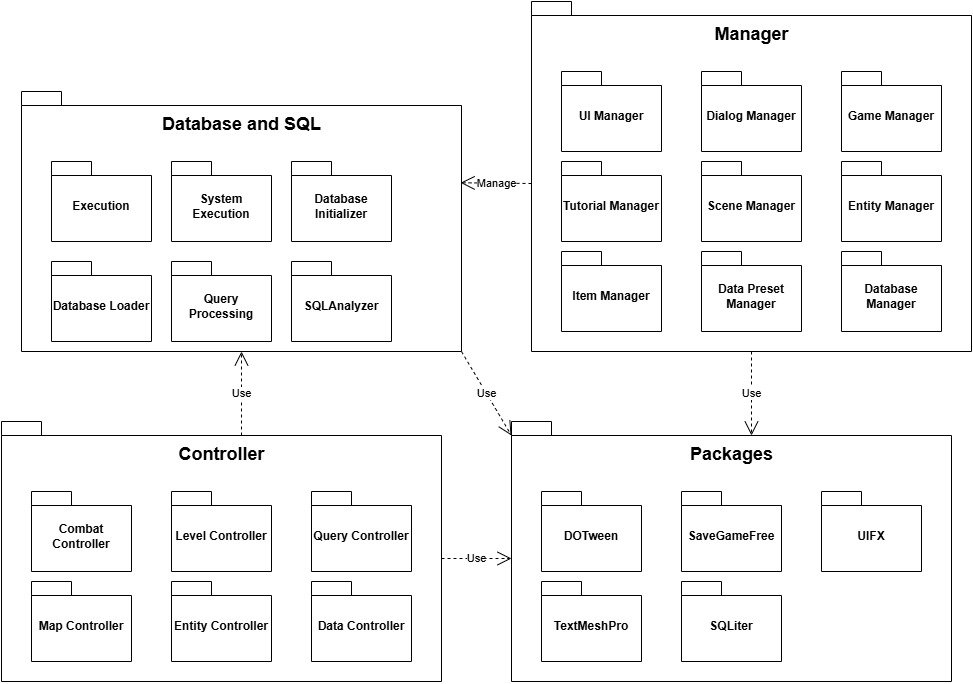
\includegraphics[width=\textwidth]{Images/Module.jpg}
	\vspace{0.5cm}
	\caption{Module chính của trò chơi}
\end{figure}
\subsection{Sequence Diagram của việc nhập câu truy vấn của người chơi}
\begin{figure}[H]
	\centering
	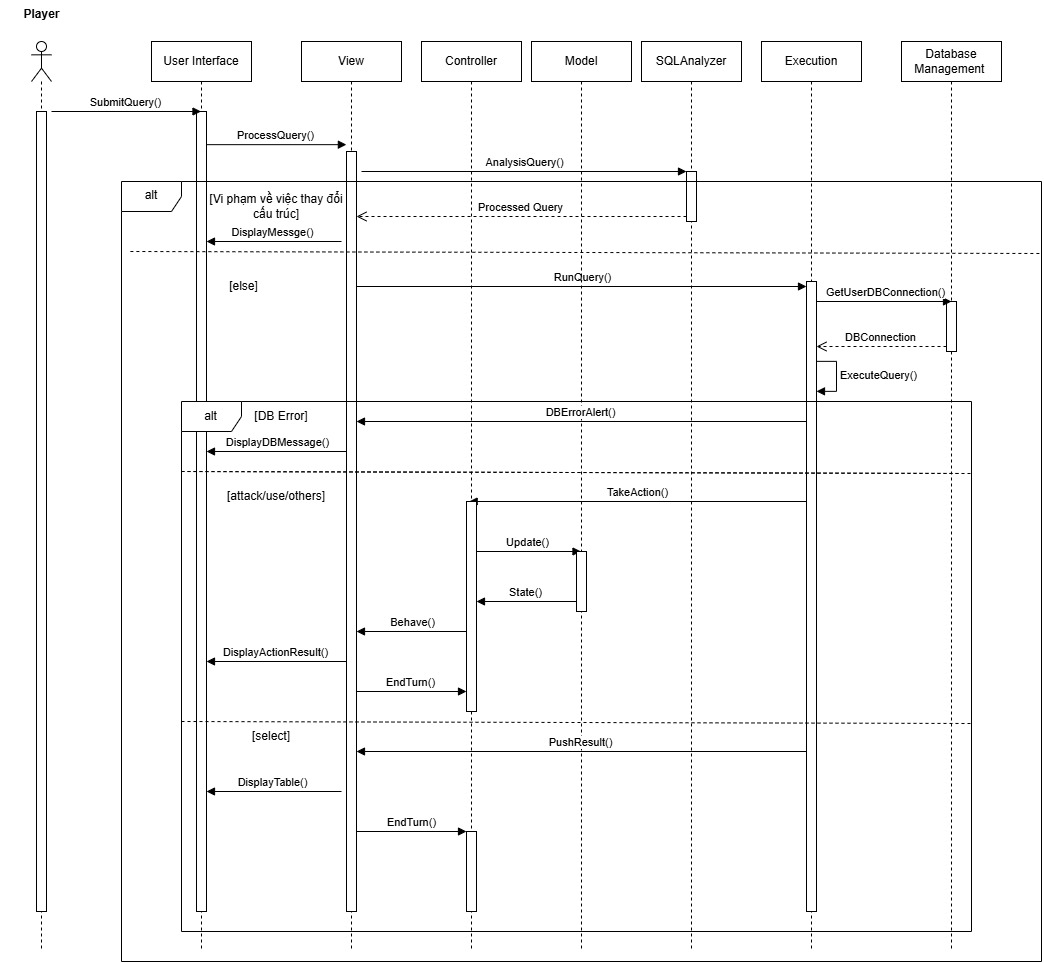
\includegraphics[width=\textwidth]{Images/seqQuery.jpg}
	\vspace{0.5cm}
	\caption{Sequence Diagram dành cho việc nhập câu truy vấn từ người chơi}
\end{figure}

